% ww-tc.tex

%%%%%%%%%%%%%%%%%%%%%%%%%%%%%%
\documentclass{standalone}
% newcommands.tex

\newcommand{\enq}{\texttt{enq}}
\newcommand{\deq}{\texttt{deq}}
\newcommand{\pput}{\texttt{PUT}}
\newcommand{\get}{\texttt{GET}}
\newcommand{\vs}{\texttt{vis}}
\newcommand{\so}{\texttt{so}}
\newcommand{\arb}{\texttt{ar}}
\newcommand{\rf}{\texttt{rf}}

% example
\newcommand{\po}[2]{\draw [->, thick] (#1) to node[above] {\Large{\so}} (#2);}
\newcommand{\pva}[2]{\draw [->, thick] (#1) to node[above] {$\Large{\so},\Large{\vs},\Large{\arb}$} (#2);}
\newcommand{\pbva}[2]{\draw [->, thick] (#1) to node[above] {$\Large{\so}$} node[below] {$\Large{\vs},\Large{\arb}$} (#2);}
\newcommand{\pv}[2]{\draw [->, thick] (#1) to node[above] {\Large{\so}} node[below] {\Large{\vs}} (#2);}
\newcommand{\evis}[2]{\draw [->, thick] (#1) to node[above, sloped, near end] {\Large{\vs}} (#2);}
\newcommand{\mvis}[2]{\draw [->, thick] (#1) to node[above, sloped] {\Large{\vs}} (#2);}
\newcommand{\ar}[2]{\draw [->, thick, allow upside down] (#1) to node[above, sloped] {\Large{\arb}} (#2);}
\newcommand{\va}[2]{\draw [->, thick, allow upside down] (#1) to node[above, sloped] {$\Large{\vs},\Large{\arb}$} (#2);}
\newcommand{\vab}[2]{\draw [->, thick, allow upside down] (#1) to node[below, sloped, near end] {$\Large{\vs},\Large{\arb}$} (#2);}
\newcommand{\vae}[2]{\draw [->, thick, allow upside down] (#1) to node[above, sloped, near end] {$\Large{\vs},\Large{\arb}$} (#2);}
\newcommand{\vas}[2]{\draw [->, thick, allow upside down] (#1) to node[sloped, near start, above] {$\Large{\vs},\Large{\arb}$} (#2);}

% serialization
\newcommand{\scc}[2]{\draw [->, very thick] (#1) to (#2);}
\newcommand{\rva}[2]{\draw [->, thick, allow upside down] (#1) to node[above, sloped] {$\Large{\rf},\Large{\vs},\Large{\arb}$} (#2);}
\newcommand{\rvb}[2]{\draw [->, thick, allow upside down] (#1) to node[below, sloped] {$\Large{\rf},\Large{\vs},\Large{\arb}$} (#2);}


\usepackage{tikz}
\usetikzlibrary{shapes, positioning, arrows.meta, decorations.pathmorphing}

\begin{document}
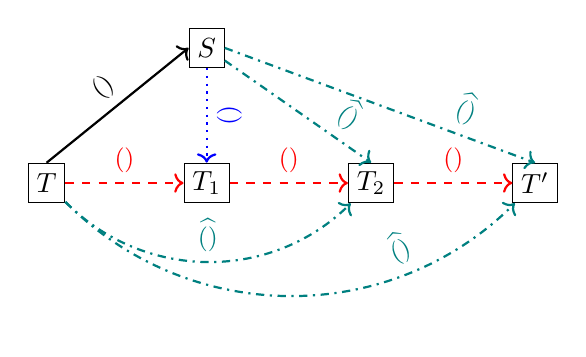
\begin{tikzpicture}[
  node distance = 1.2cm and 1.5cm,
  wr/.style = {->, thick, font = \small},
  ww/.style = {->, thick, dashed, red, font = \small},
  wwhat/.style = {->, thick, dash dot, teal, font = \small},
  rw/.style = {->, thick, dotted, blue, font = \small},
  rwhat/.style = {->, thick, dash dot, teal, font = \small},
  txn/.style = {draw, inner sep = 3pt, minimum height = 0.5cm, align = center}]

  \node[txn] (t) {$T$};
  \node[txn, right = of t] (t1) {$T_{1}$};
  \node[txn, right = of t1] (t2) {$T_{2}$};
  \node[txn, right = of t2] (t3) {$T'$};

  \node[txn, above = of t1] (s) {$S$};

	% ww
	\draw[ww] (t) to node[above]{$\WW(\keyxvar)$} (t1);
	\draw[ww] (t1) to node[above]{$\WW(\keyxvar)$} (t2);
	\draw[ww] (t2) to node[above]{$\WW(\keyxvar)$} (t3);

	% ww-hat
	\draw[wwhat, sloped, bend right = 45] (t) to
	  node[above]{$\widehat{\WW(\keyxvar)}$} (t2);
	\draw[wwhat, sloped, bend right = 45] (t) to
	  node[above, near end]{$\widehat{\WW(\keyxvar)}$} (t3);

	% wr
	\draw[wr, sloped] (t.north) to
	  node[above]{$\WR(\keyxvar)$} (s.west);

	% rw
	\draw[rw, sloped] (s.south) to
	  node[above]{$\RW(\keyxvar)$} (t1.north);
	% rwhat
	\draw[rwhat, sloped] (s) to
	  node[above, near end]{$\widehat{\RW(\keyxvar)}$} (t2.north);
	\draw[rwhat, sloped] (s.east) to
	  node[above, near end]{$\widehat{\RW(\keyxvar)}$} (t3.north);

  % \draw[wr, sloped] (t1) to node[above]{$\WR(\keyxvar)$} (t2.west);
  % \draw[ww, sloped, bend left = 45] (t1) to node[above]{$\WW(\keyxvar)$} (t2);

  % \draw[wr, sloped] (t1) to node[below]{$\WR(\keyxvar)$} (t3.west);
  % \draw[ww, sloped, bend right = 45] (t1) to node[below]{$\WW(\keyxvar)$} (t3);

  % \draw[rw, sloped, near start] (t2.-160) to node[below]{$\RW(\keyxvar)$} (t3.20);
  % \draw[rw, sloped, near end] (t3.160) to node[below]{$\RW(\keyxvar)$} (t2.-20);
\end{tikzpicture}
\end{document}
%%%%%%%%%%%%%%%%%%%%%%%%%%%%%%